\chapter{Discrete state adaptive network models}

In this chapter, the swarming systems class of adaptive network models with a discrete state set will be introduced. We will consider the same types of networks as developed by Chen \textit{et al.} \cite{Chen2016}.

\section{Network topology and dynamics}

A network can be represented by a graph which consists of $N$ discrete nodes, representing agents. Each node has an internal state and the set of all possible states is denoted by $\Omega$. In this chapter, we take a discrete state set $\Omega = \{1,2,...,M\}$ containing $M$ possible states. Nodes may be connected to multiple other nodes by links, indicating mutual awareness of the corresponding agents. 

For example when applying the network as a voter model, where all individuals in a population have to answer a certain question with either 'yes' or 'no', each node represents a different person holding one of the opinions contained in the state set $\Omega = \{\text{yes}, \text{no}\}$. People who talk about their opinion on a regular basis would be connected by a link. As a second example, we can consider the swarming motion of self-propelled particles in two-dimensional space, with constant speed. This can be modelled by having the nodes represent particles with their state corresponding to their direction, contained in $\Omega = \{\text{up}, \text{down}, \text{left}, \text{right}\}$. Particles who are aware of each other's direction are connected by a link. 

Having defined the network properly, we can impose dynamical rules on the network such that it is able to evolve in time. Analogous to \cite{Chen2016}, we distinguish four types of dynamics:
\begin{description}
	\item [Type 1] Nodes change spontaneously to another uniformly chosen state with rate $\eta$.
	\item [Type 2] In a triplet of nodes in configuration X-Y-X, where a node in state Y is connected to two nodes in state X, the middle node takes the state of its two neighbours such that it ends up in an X-X-X configuration with rate $\sigma_d$ per triplet. 
	\item [Type 3] Links are created between two arbitrary not-linked nodes occupying different states with rate $\alpha$ per pair.
	\item [Type 4] Links are removed between two arbitrary linked nodes occupying different states with rate $\beta$ per link.
\end{description}
The first two types are referred to as state dynamics since they influence the internal state of the nodes, whilst the latter two change the topology of the network by rewiring links and therefore they are referred to as link dynamics. All four types of dynamics are visualised in \cref{fig:dynamics_discrete} and take place irrespective of any additional links that the nodes may have. 
\begin{figure}[t]
	\centering
	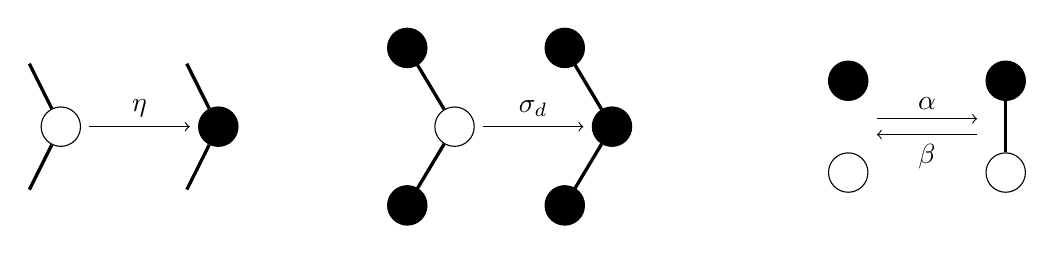
\begin{tikzpicture}[rotate=0]
	
	\draw[] (-5,0) node[circle, minimum size =0.5cm, draw] (state11) {};
	\draw[] (-3,0) node[circle, fill=black, minimum size =0.5cm, draw] (state12) {};
	
	\draw[->, shorten <=3pt, shorten >=3pt] (state11)--(state12) node[above, xshift=-1cm] {$\eta$};
	\draw[very thick] (state11)--(-5.4,0.8);
	\draw[very thick] (state11)--(-5.4,-0.8);
	\draw[very thick] (state12)--(-3.4,0.8);
	\draw[very thick] (state12)--(-3.4,-0.8);
	
	%%%%%%%%%%%%%%%%
	
	
	\draw[] (0,0) node[circle, minimum size =0.5cm, draw] (state21) {};
	\draw[] (-0.6,-1) node[circle, fill=black,minimum size =0.5cm, draw] () {};
	\draw[] (1.4,-1) node[circle, fill=black,minimum size =0.5cm, draw] () {};
	\draw[] (2,0) node[circle, fill=black, minimum size =0.5cm, draw] (state22) {};
	\draw[] (-0.6,1) node[circle, fill=black,minimum size =0.5cm, draw] () {};
	\draw[] (1.4,1) node[circle, fill=black,minimum size =0.5cm, draw] () {};
	
	\draw[->, shorten <=3pt, shorten >=3pt] (state21)--(state22) node[above, xshift=-1cm] {$\sigma_d$};
	\draw[very thick] (state21)--(-0.6,-1);
	\draw[very thick] (state21)--(-0.6,1);
	\draw[very thick] (state22)--(1.4,-1);
	\draw[very thick] (state22)--(1.4,1);
	
	%%%%%%%%%%%%%%%%%%
	
	\draw[] (7,0.583) node[circle, fill=black, minimum size =0.5cm, draw] (link11) {};
	\draw[] (5,0.583) node[circle, fill=black, minimum size =0.5cm, draw] (link12) {};
	\draw[] (7,-0.583) node[circle, minimum size =0.5cm, draw] (link13) {};
	\draw[] (5,-0.583) node[circle, minimum size =0.5cm, draw] (link14) {};
	
	\draw[very thick] (link11)--(link13);

	\draw[->, shorten <=3pt, shorten >=3pt, transform canvas={yshift=-0.683cm}] (link11)--(link12) node[below, xshift=1cm] {$\beta$};
	\draw[->, shorten <=3pt, shorten >=3pt, transform canvas={yshift=-0.483cm}] (link12)--(link11) node[above, xshift=-1cm] {$\alpha$};

	\end{tikzpicture}
	\caption{Illustration of the model, four types of dynamics are applied to the discrete state adaptive network models. The internal state of each node (circle) is represented by its colour. These dynamics take place irrespective of any additional links that may be present, but are not drawn.}
	\label{fig:dynamics_discrete}
\end{figure}

\section{Counting of motifs}

In this section, we will formalise different quantities that are used throughout the first part of this thesis, in particular the density of nodes in a certain state, densities of links and small subgraphs and how these motifs are counted in the network. Unfortunately, these are not unambiguously defined in literature, hence, to be absolutely clear in this work, we will write down all definitions explicitly. This section is based on \cite{Chen2016, Demirel2014} and personal email communication with dr T. Gross \cite{GrossMail}.

The adaptive network model is developed with the use of different motif densities. First, we define the density of nodes

\begin{definition}
	Let $X\in\Omega$. The density of nodes in state $X$, $\X$, is the total number of nodes in state X, $N_X$, normalised against the total number of nodes in the network $N$, i.e. $\X=\frac{N_X}{N}$.
\end{definition}

Note that we have $\X\in [0,1]$ for all $X \in \Omega$ and $\sum\limits_{X\in\Omega} \X =1$.

\begin{definition}
	Let $X,Y\in\Omega$. The density of links $\XY$, connecting a node in state $X$ to a node in state $Y$ (XY-links) is the total number of XY-links $N_{XY}$ normalised against the total number of nodes in the network $N$, i.e. $\XY = \frac{N_{XY}}{N}$.
\end{definition}

This means that the links are not double counted, so if we have a network with one $XX$-link, it is counted as $\frac{1}{N}$. In other words, we do \textit{not} check for each $X$-node to how many other $X$-nodes it is connected, but we really count the links connecting certain nodes. Note that some papers do this differently although they do not always mention this clearly.  Furthermore note that the link density is symmetric, that is, $\XY = [YX]$ for $X,Y\in\Omega$. 

\begin{definition}
	Let $X,Y,Z\in\Omega$. The density of triplets $\XYZ$ connecting a node in state $Y$ to a node in state $X$ and to a node in state $Z$ (XYZ-triplets) is the total number of XYZ-triplets $N_{XYZ}$ normalised against the total number of nodes in the network $N$, i.e. $\XYZ = \frac{N_{XYZ}}{N}$.
\end{definition}

Throughout this work, we assume that the density of triangular triplets is low enough such that they are described accurately enough by the line-like triplets. Therefore we do not need a separate density for triangular configurations. However, in dealing with highly clustered networks these triangles do need to be taken into account. Keeling \cite{Keeling1999} describes how to deal with these and other clustering effects. Moreover, note that also triplet densities are symmetric, such that $[XYZ] = [ZYX]$, but $[XYZ] \ne [XZY]$.

\begin{definition}
	Let $W,X,Y,Z\in\Omega$. The density of four-body subgraphs $\XYZW$ connecting a node in state $Y$ to nodes in state $W, X$ and $Z$, is the total number of subgraphs in this configuration $N_{^XY_W^Z}$ normaised against the total number of nodes in the network $N$, i.e. $[XYZW]=\frac{N_{^XY_W^Z}}{N}$. 
\end{definition}

There is again a symmetry relation: $[^XY_W^Z] = [^XY_Z^W] = [^ZY_X^W]=[^ZY_W^X] = [^WY_Z^X] = [^WY_X^Z]$, as long as the middle node is in state $Y$. In addition, note that there are no conservation laws for the link, triplet and four-body subgraph densities.

\begin{example}
	\label{ex:config_example}
	Let $X,Y,Z\in\Omega$. Suppose we have a triangular configuration of nodes in states $X,Y$ and $Z$. Furthermore suppose an extra node in state $X$ is connected to the node in state $Y$, see \cref{fig:config_example}. Then we have $\X = \frac{2}{4}$,  $\Y = [Z] = \frac{1}{4}$, $[XZ]=[ZX]=\frac{1}{4}$, $[XY] = [YX] = \frac{2}{4}$, $[XYX]=\frac{1}{4}$, $[XYZ]=[ZYX]= \frac{2}{4}$, $[YXZ]=\frac{1}{4}$ and $[^XY_X^Z]=\frac{1}{4}$, all normalised against the number of nodes in the network $N=4$.
\end{example}
\begin{figure}[tphb]
	\centering
	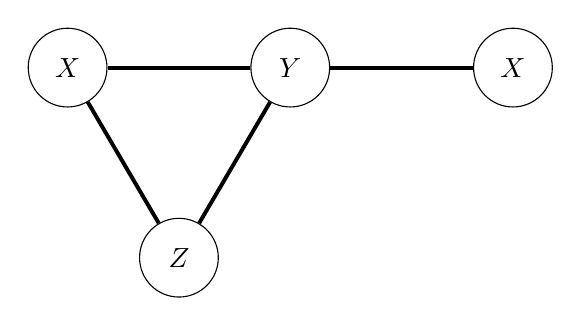
\begin{tikzpicture}[scale=0.5,rotate=0]
	\draw[] (0,-2) node[circle,minimum size=1cm, draw] (Zunder) {$Z$};
	\draw[] (2*1.414, 2*1.414) node[circle,minimum size=1cm, draw] (Ymiddle) {$Y$};
	\draw[] (2*-1.414, 2*1.414) node[circle,minimum size=1cm, draw] (Xleft) {$X$};
	\draw[] (6*1.414, 2*1.414) node[circle,minimum size=1cm, draw] (Xright) {$X$};

	\draw[line width=0.5mm] (Zunder) -- (Ymiddle);
	\draw[line width=0.5mm] (Zunder) -- (Xleft);
	\draw[line width=0.5mm] (Ymiddle) -- (Xleft);
	\draw[line width=0.5mm] (Ymiddle) -- (Xright);	
	\end{tikzpicture}%
	\caption{Configuration considered in \cref{ex:config_example}. A triangular configuration of nodes in states $X,Y$ and $Z$, in which the node in state $Y$ is connected to an additional node in state $X$.}
	\label{fig:config_example}
\end{figure}

With these definitions we can derive a set of ordinary differential equations (ODEs), which describes the time evolution of the network. As this is done in \cite{Chen2016}, we will omit writing out the derivation. The resulting system describing the discrete state adaptive network models can be written as

\begin{adjustwidth}{-.5in}{-.5in} 
\small
\begin{subequations}
\label{eq:discrete_system}
\begin{alignat}{1}
\frac{d}{dt}\X 
&= \frac{\eta}{M-1} \left[ \sum_{Y\in\Omega\setminus\{X\}}\Y-(M-1)\X\right] + \sigma_d \sum_{Y\in\Omega\setminus\{X\}} \left( \XYX - [YXY] \right), \label{eq:discrete_system1} \\
\frac{d}{dt}\XX 
&= \frac{\eta}{M-1} \left[\sum_{Y\in\Omega\setminus\{X\}}\XY -2(M-1)\XX \right] + \sigma_d \sum_{Y\in\Omega\setminus\{X\}} \left( 2\XYX + 3[^XY^X_X] - [^XX_Y^Y] \right), \label{eq:discrete_system2} \\
\frac{d}{dt} [XX'] 
&= \frac{\eta}{M-1} \left[2 (\XX + [X'X']) + \sum_{Y\in\Omega\setminus\{X, X'\}} \left( \XY + [X'Y]\right)  -2(M-1)[XX'] \right] \label{eq:discrete_system3}\\ 
&\quad + \sigma_d \ \Bigg[ -2[XX'X] -2[X'XX'] + [^{X}X^{X'}_{X'}] + [^{X'}X'^{X}_{X}] -3[^{X'}X^{X'}_{X'}] -3[^{X}X'^{X}_{X}] \Bigg] \nonumber \\ 
&\quad  + \sigma_d \  \sum_{Y\in\Omega\setminus\{X, X'\}} \Bigg[ [^{X'}Y^{X}_{X}] + [^{X}Y^{X'}_{X'}] - [^{X}X^{Y}_{Y}] - [^{X'}X^{Y}_{Y}] \Bigg] \nonumber\\ 
&\quad + \alpha \X[X'] - \beta [XX'].\nonumber
 \end{alignat}
\end{subequations}
\end{adjustwidth}
\normalsize
where $X,X'\in\Omega$, with $X\ne X'$. This system represents a bigger number of equations, since we have similar expressions for $\frac{d}{dt}\Y, \frac{d}{dt}\YY$ etcetera. The complete system consists of $M(2+\frac{1}{2}(M-1))$ equations. 
The coefficients in the equations can be explained by the symmetry relations. For example, $\frac{d}{dt} [XX']$ depends on $\frac{2\eta}{M-1} [XX]$, since either of the two nodes in state $X$ may change to state $X'$ with rate $\frac{\eta}{M-1}$, creating an $XX'$-link. As a second example, $\frac{d}{dt} [XX']$ depends on $\sigma_d (-2[X'XX'] + [^XX^{X'}_{X'}])$, since if the middle $X$-node changes to state $X'$, two $XX'$-links are lost in the $X'XX' $-triplet. However, if the middle node in the triplet happens to be connected to another $X$-node, an extra $XX'$-link is created, resulting in an overall loss of one $XX'$-link.

Notice that this system is not closed. That is, not all terms are known. All moment equations of a given order are dependent on higher order terms. One might think this means we need extra equations for these higher order moments, but this would lead to a great hierarchy of connected ODEs which would be very hard to solve. Moreover, numerical estimates would not allow developing an analytical solution \cite{Demirel2014}. This can be prevented in multiple ways. In the next sections two possibilities are described: the mean field approximation and the moment closure approximation.  


\section{Mean field approximation}
In the previous sections, the topology of and dynamics on the adaptive networks were considered.  In this section, we will look at the most simple model which describes the time evolution of such a network: the mean field approximation. Although this approximation omits a lot of the properties of the described network, it gives a good qualitative description of how the network develops. A more accurate model, which also closes the system of equations, is described in the next section. 

In the mean field approximation we consider a network in which we neglect link dynamics (type 3 and 4). Moreover, it is assumed that the density of links connecting nodes in a given state is proportional to the product of the densities of these states, where the proportionality constant is given by $\langle k \rangle$, the mean degree of the network. In other words, we express the link densities in terms of the node densities, e.g. $\XY = \langle k \rangle \X\Y$.  Suppose $\Omega = \{1,2,...M\}$ such that we have an $M$-state system in which $\X$ is the density of nodes in state $X\in\Omega$ as a function of continuous time $t$. Furthermore we denote the density of all other $M-1$ states by $\Yi$, $i \in \{1,2,...,M-1\}$. The time evolution of $\X$ can now be described as 
\begin{equation}
	\frac{d}{dt}\X = \frac{\eta}{M-1} \left( \sum\limits_{i=1}^{M-1} \Yi \right) - \eta\X + \sigma_d \langle k \rangle ^2 \sum\limits_{i=1}^{M-1} (\X^2\Yi - \Yi^2 \X).
\end{equation}
Numerical simulations in \cite{Chen2016} suggest that the system converges either to a disordered solution in which all densities are equal, or to an ordered state in which one single state dominates and all other states have the same lower density. Using this, let us assume $[Y_1] = [Y_2] = ... = [Y_{M-1}] \coloneq \Y$, such that the system simplifies to 
\begin{equation}
\frac{d}{dt}\X = \eta (\Y-\X) + \sigma_d \langle k \rangle ^2 (M-1) (\X^2\Y - \Y^2 \X).
\end{equation}
The steady state solutions can be obtained by setting $\frac{d}{dt}\X =0$. This yields
$
	\X=\Y=\frac{1}{M}
$
and
$
	\X = \frac{1}{2} \pm \sqrt{\frac{1}{4} - \frac{\eta}{\sigma_d \langle k \rangle ^2}},
$
where the latter is independent of the number of states $M$. These results are in accordance with the results found in \cite{Chen2016}.

\section{Moment closure approximation}

In this section, the second way of closing the system im \cref{eq:discrete_system} is considered, which is a moment closure approximation. This means that higher order terms are approximated using the known lower order terms. Various closure approximations are discussed by Demirel \textit{et al.} \cite{Demirel2014}. In this work we use the homogeneous pair approximation.

\subsection{Triplets}

Let us suppose that the highest densities known are link densities and we want to find an expression for triplet densities in terms of these link densities and node densities. That is, we want to find for instance a function $f$ such that $\XYX = f(\Y, \XY)$. In order to find $f$, first suppose we have an XY-link with density $\XY$, moreover assume that the XY-links are uncorrelated\footnote{We do need to assume that the Y-node has a higher than average degree since we already know it is connected to an $X$-node \cite{Demirel2014}.}. Now each of the additional links connected to the Y-node in the existing link is an XY-link with probability 
\begin{equation}\small
	P_{X}=P(\text{additional X connected to the Y | XY-link})=\frac{\XY}{\XY + 2\YY + \ZY + ...}=\frac{\XY}{\Y \langle k_Y \rangle},
\end{equation}\normalsize
in which $\langle k_Y \rangle$ represents the mean degree of nodes occupying state $Y$. The factor 2 comes from the fact that the YY-link may be connected on either side to the Y-node in the XY-link. 

Now to create an XYX-triplet, we need to multiply the existing XY-link density by the expected number of additional links of the Y-node $\langle q_Y \rangle$ and by the probability $P_{X}$ of the additional link being an XY-link. This yields
\begin{equation}
	\XYX = \frac{1}{2} \XY \langle q_Y \rangle P_{X} = \frac{1}{2} \frac{\langle q_Y \rangle}{\langle k_Y \rangle} \frac{\XY^2}{\Y}
\end{equation}
The factor of $\frac{1}{2}$ comes from the fact that we need to correct for double counting. To explain this compare this derivation to counting the number of possible links in a network of $N$ nodes. One might expect that the amount of possible links equals $N(N-1)$, but then every link would be counted twice. The actual number of possible links is $\frac{1}{2}N(N-1)$. For creating triplets there is a similar situation. Suppose we have four XY-pairs, then there are six potential triplets. This is visualised in \cref{fig:counting_triplets_double}. However, $N_{XY}(N_{XY}-1) = 12$. Hence, the factor of $\frac{1}{2}$ is needed to correct for double counting. In the networks, we assume that the number of triplets is high enough that we can neglect the `$-1$', justifying the derived closure equation.

\begin{figure}[htp]
	\centering
	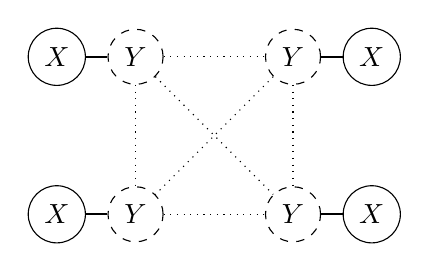
\begin{tikzpicture}[rotate=0]
	\draw[] (-2,1) node[circle,minimum size=0.5cm,draw] (tll) {$X$};
	\draw[dashed] (-1,1) node[circle,minimum size=0.5cm,draw] (tl) {$Y$};
	\draw[] (-2,-1) node[circle,minimum size=0.5cm,draw] (bll) {$X$};
	\draw[dashed] (-1,-1) node[circle,minimum size=0.5cm,draw] (bl) {$Y$};
	
	\draw[] (2,1) node[circle,minimum size=0.5cm,draw] (trr) {$X$};
	\draw[dashed] (1,1) node[circle,minimum size=0.5cm,draw] (tr) {$Y$}; 
	\draw[] (2,-1) node[circle,minimum size=0.5cm,draw] (brr) {$X$};
	\draw[dashed] (1,-1) node[circle,minimum size=0.5cm,draw] (br) {$Y$};
	
	\draw[thick] (tll) -- (tl);
	\draw[thick] (trr) -- (tr);
	\draw[thick] (bll) -- (bl);
	\draw[thick] (brr) -- (br);
	
	\draw[dotted] (tl) -- (tr);
	\draw[dotted] (tl) -- (br);
	\draw[dotted] (tl) -- (bl);
	\draw[dotted] (tr) -- (bl);
	\draw[dotted] (tr) -- (br);
	\draw[dotted] (bl) -- (br);

	\end{tikzpicture}
	\caption{Four XY-pairs create six potential triplets.}
	\label{fig:counting_triplets_double}
\end{figure}


The quantity $\frac{\langle q_Y \rangle}{\langle k_Y \rangle}$ is not known in general since it depends on the exact network topology, which changes in time due to link dynamics \cite{Demirel2014}. However, on random graphs created by the Erdös-Rényi model \cite{Erdos1959} it turns out that assuming $\langle q_Y \rangle = \langle k_Y \rangle$ yields good results if the degree distribution is not too wide \cite{Gross2006}.

In a similar fashion, we can derive 
\begin{equation}
	\XYY = 2 \frac{\langle q_Y \rangle}{\langle k_Y \rangle} \frac{\XY\YY}{\Y},
\end{equation}
only this time there is a factor 2 which comes from the fact that each YY-pair may be connected to the X on either side. We do not need the factor of $\frac{1}{2}$ since in combining XY- and YY-pairs we do not double count XYY-triplets. 

Lastly, we can also derive
\begin{equation}
	\XXX = 2 \frac{\langle q_X \rangle}{\langle k_X \rangle} \frac{\XX^2}{\X},
\end{equation}
in which both effects occur. We need a factor of $\frac{1}{2}$ to correct for double counting, but we also need two factors of 2 since both XX-pairs may be connected on either side. This results in an overall factor of 2. 

Taking all these effects together and assuming $\langle q_X \rangle=\langle k_X \rangle$ we generalise the triplet closure by writing an arbitrary density $\XYZ$ as 
\begin{equation}
	\XYZ = \frac{(1+\delta_{XY})(1+\delta_{YZ})}{1+\delta_{XZ}} \frac{\XY\YZ}{\Y},
	\label{eq:closure_discrete_3}
\end{equation}
with $\delta$ the Kronecker delta.

\subsection{Four-body subgraphs}
Since the density of four-body subgraphs is also unknown we will find a function $g$ such that $\XYZW = g(\XYZ, \YW, \Y)= g(f(\XY, \YZ, \Y), \YW, \Y)$. The same reasoning as with the triplets can be used to find $g$.

Suppose we already have an XYZ-triplet and each of the additional links of the Y node is a YW link with probability 
\begin{equation}
	P_{YW}=P(\text{YW link | XYZ triplet}) = \frac{\YW}{\YW + 2\YY + \ZY + \XY + ...} = \frac{\YW}{\Y \langle k_Y \rangle}.
\end{equation}

In order to create an XYZW-triplet, we need to multiply the existing XYZ-link density (approximation) by the expected number of additional links of the Y node $\langle q_Y \rangle -1$ (under the condition it is already connected to an X and a Z node) and by the probability $P_{YW}$ of the additional link being a YW-link. Neglecting the `$-1$', the result is
\begin{equation}
	\begin{aligned}
		\XYZW &= \XYZ (\langle q_y \rangle -1) P_{YW} \\
	%	&= \frac{(1+\delta_{XY})(1+\delta_{YZ})}{1+\delta_{XZ}} \frac{\XY\YZ}{\Y} %\frac{\langle q_y \rangle -1}{\langle k_Y \rangle} \frac{\YW}{\Y}\\
		&= \frac{(1+\delta_{XY})(1+\delta_{YZ})(1+\delta_{YW})}{1+\delta_{XZ}+\delta_{XW}+\delta_{ZW}+\delta_{XZ}\delta_{ZW}+\delta_{XW}\delta_{ZW}}\frac{\XY\YZ\YW}{\Y^2},
	\end{aligned}
	\label{eq:closure_discrete_4}
\end{equation}

where all delta functions correct for aforementioned effects of double counting and symmetry. Again we made use of the assumption $\langle q_X \rangle=\langle k_X \rangle $.


\subsection{Closing the system of ODEs}
The derived moment closure approximations can now be used to close the system of ordinary differential equations, by substitution of \cref{eq:closure_discrete_3} and \cref{eq:closure_discrete_4} into \cref{eq:discrete_system}. For more information on the quality of the closure relations and special situations in which they may be a less suitable approximation, one can read \cite{Demirel2014}. In the rest of this thesis, we will assume these relations to be valid for the considered discrete state adaptive networks.